\documentclass[
    NAME={Dr. Helga Ingimundardóttir},
    EMAIL={helgaingim@hi.is},
    FACULTY={Industrial Engineering},
    TITLE={Nonlinear Optimization},
    SUBTITLE={Approaches and Challenges},
    SEMINAR={VÉL113F},
    DATE={Design and Optimization}
]{../HI-latex/hi-beamer}
\let\oldframe\frame
\renewcommand\frame[1][allowframebreaks]{\oldframe[#1]}

% Define new commands for nested itemize
\newcommand{\bi}{\begin{itemize}
                     \item}
\newcommand{\ei}{\end{itemize}}

\usepackage{IEEEtrantools}

\usepackage{algorithm}
\usepackage{algpseudocode}

% use mathbf instead of vec
\renewcommand{\vec}[1]{\ifmmode\text{\boldmath$#1$}\else\textbf{#1}\fi}
\newcommand{\mat}[1]{\mathbf{#1}}

\begin{document}

    \begin{frame}{Introduction}
        \begin{block}{Nonlinear optimization}
            Unlike linear optimization, nonlinear optimization deals with problems where the objective function \emph{or}
            the constraints are nonlinear functions, making the solutions more complex.
        \end{block}
    \end{frame}


    \section{Basic Concepts}
    \begin{frame}{Basic Concepts}
        \begin{block}{Definition:}
            Nonlinear optimization focuses on finding the best solution to a problem where
            either the objective function, the constraints, or both are nonlinear.
        \end{block}
        \begin{itemize}

            \item \emph{Objective Function:} Function that needs to be optimized, which can be either maximized or
            minimized.

            \item \emph{Constraints:} Restrictions or limitations imposed on the solution.

            \item \emph{Feasible Region:} Set of all solutions that satisfy the constraints.

            \item \emph{Optimal Solution:} Best possible solution from the set of feasible solutions.

            \item \emph{Local vs. Global Optima:} Understanding the difference between local optima (best solution
            in a neighborhood) and global optima (best solution overall).

            \item \emph{Convexity:} A function is convex if the line segment between any two points on the function
            lies above or on the function. Important for the convergence of certain algorithms.

            \item \emph{Gradient and Hessian:} First and second derivatives, respectively, essential in determining
            the nature of the optimum (minimum, maximum, or saddle point).
        \end{itemize}
        \begin{figure}
            \centering
            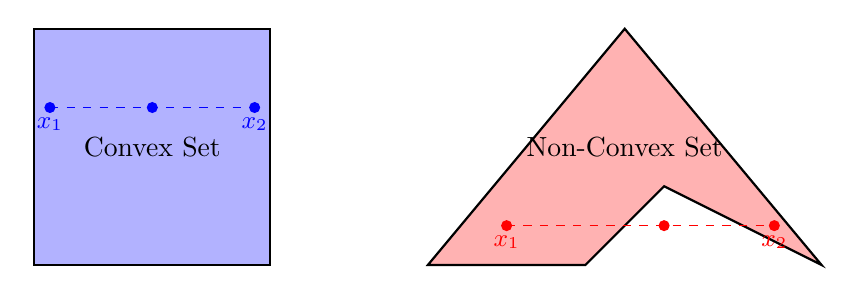
\begin{tikzpicture}
                % Convex Set
                \fill[blue!30] (0,0) -- (0,3) -- (3,3) -- (3,0) -- cycle;
                \draw[thick] (0,0) -- (0,3) -- (3,3) -- (3,0) -- cycle;
                \draw (1.5,1.5) node {Convex Set};

                % Non-Convex Set
                \fill[red!30] (5,0) -- (7.5,3) -- (10,0) -- (8,1) -- (7,0) -- cycle;
                \draw[thick] (5,0) -- (7.5,3) -- (10,0) -- (8,1) -- (7,0) -- cycle;
                \draw (7.5,1.5) node {Non-Convex Set};

                % Lines for illustration
                \draw[blue,dashed] (.2,2) -- (2.8,2);  % This lies entirely within the convex set
                \fill[blue] (.2,2) circle (2pt);  % left endpoint
                \node[blue, below, font=\small] at (.2, 2) {\(x_1\)};
                \fill[blue] (2.8,2) circle (2pt);  % right endpoint
                \node[blue, below, font=\small] at (2.8, 2) {\(x_2\)};
                \fill[blue] (1.5,2) circle (2pt); % center point

                \draw[red,dashed] (6,.5) -- (9.4,.5); % This does not lie entirely within the non-convex set
                \fill[red] (6,.5) circle (2pt);  % left endpoint
                \node[red, below, font=\small] at (6, .5) {\(x_1\)};
                \fill[red] (9.4,.5) circle (2pt); % right endpoint
                \node[red, below, font=\small] at (9.4, .5) {\(x_2\)};
                \fill[red] (8,.5) circle (2pt); % center point

            \end{tikzpicture}
            \caption{Convex and non-convex sets.}
        \end{figure}
    \end{frame}
    \begin{frame}{Example of Non-linear Optimization}
        \begin{eqnarray*}
            \text{maximize}   & & x_1 + x_2 \\
            \text{subject to} & & x_1 \geq 0,  x_2 \geq 0 \\
            & & x_1^2 + x_2^2 \geq 1 \\
            & & x_1^2 + x_2^2 \leq 2 \\
        \end{eqnarray*}
        \begin{figure}
            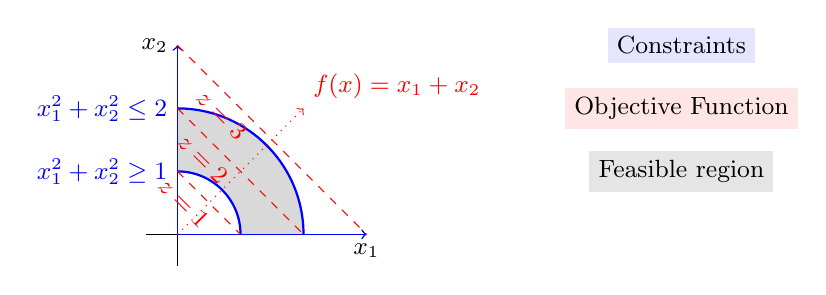
\begin{tikzpicture}[scale=0.8,every node/.style={font=\small}]
                % Feasible region between two half circles
                \fill[gray!30] (0,0) -- (2,0) arc (0:90:2) -- cycle; % Half circle with radius 2
                \fill[white] (0,0) -- (1,0) arc (0:90:1) -- cycle; % Half circle with radius 1 to overlay on the gray region

                % Axes
                \draw[->] (-0.5,0) -- (3,0) node[anchor=north] {$x_1$};
                \draw[->] (0,-0.5) -- (0,3) node[anchor=east] {$x_2$};
                \draw[blue,->] (0,0) -- (3,0);
                \draw[blue,->] (0,0) -- (0,3);

                % Constraints
                \draw[blue,thick] (1,0) arc (0:90:1) node[at end, left] {$x_1^2 + x_2^2 \geq 1$};
                \draw[blue,thick] (2,0) arc (0:90:2) node[at end, left] {$x_1^2 + x_2^2 \leq 2$};

                % Objective function
                \draw[dotted, red, ->] (0,0) -- (2,2) node[anchor=south west] {$f(x) = x_1 + x_2$};

                % Contour lines for z
                \draw[dashed, red] (0,1) -- (1,0) node[pos=0.3, below, sloped] {$z=1$};
                \draw[dashed, red] (0,2) -- (2,0) node[pos=0.3, below, sloped] {$z=2$};
                \draw[dashed, red] (0,3) -- (3,0) node[pos=0.3, below, sloped] {$z=3$};
                % This will be partially outside the shown region but is included for clarity


                \node at (8,3) [rectangle,fill=blue!10] {Constraints};
                \node at (8,2) [rectangle,fill=red!10] {Objective Function};
                \node at (8,1) [rectangle,fill=gray!20] {Feasible region};

            \end{tikzpicture}
        \end{figure}

    \end{frame}


    \section{Lagrange Multipliers and the Lagrangian Function}
    \begin{frame}{Method of Lagrange Multipliers}
        \begin{block}{Method of Lagrange Multipliers}
            Technique to find the extrema of a function \( f(\mathbf{x}) \) where
            \( \mathbf{x} \in \mathbb{R}^n \), subject to constraints:
            \[ \text{optimize } f(\mathbf{x}) \text{ subject to } g(\mathbf{x}) = 0 \]

            The necessary condition for an extremum at \( \mathbf{x^*} \) is that the gradient vectors of \( f \) and \( g \) are parallel at \( \mathbf{x^*} \):
            \[ \nabla f(\mathbf{x^*}) = \lambda \nabla g(\mathbf{x^*}) \]

            This leads to a system of equations:
            $ \frac{\partial f}{\partial x_i} - \lambda \frac{\partial g}{\partial x_i} = 0, \quad \text{for } i = 1
            , \ldots , n $.

            With the additional constraint $ g(\mathbf{x}) = 0 $.
        \end{block}
        \framebreak
        \alert{Specific \( n=2 \) case:}
        For the function \( f(x_1, x_2) \) with constraint \( g(x_1, x_2) = 0 \):
        \[ \left( \frac{\partial f}{\partial x_1} - \lambda \frac{\partial g}{\partial x_1} \right) \Bigg|_{(x_1^*,x_2^*)} = 0 \]
        \[ \left( \frac{\partial f}{\partial x_2} - \lambda \frac{\partial g}{\partial x_2} \right) \Bigg|_{(x_1^*,x_2^*)} = 0 \]
        Along with:
        \[ g(x_1^*, x_2^*) = 0 \]

        For a solution to exist, the partial derivatives must be non-zero to define \( \lambda \).
    \end{frame}

    \begin{frame}{Lagrangian Function}
        Continuing from the Method of Lagrange Multipliers, a more general approach involves the use of the
        \emph{Lagrangian function}, denoted by \(L\):
        \[ L(x_1,x_2,\lambda) = f(x_1,x_2)+\lambda g(x_1,x_2)\]

        To find the conditions for an extremum, consider $L$ as a function of the variables $x_1, x_2$, and $\lambda$.
        The necessary conditions are derived by taking the partial derivatives of $L$ with respect to each
        variable and setting them to zero:
        \begin{align*}
            \frac{\partial L}{\partial x_1}(x_1,x_2,\lambda) &= \frac{\partial f}{\partial x_1}(x_1,x_2)+\lambda\frac{\partial g}{\partial x_1}(x_1,x_2) &= 0 \\
            \frac{\partial L}{\partial x_2}(x_1,x_2,\lambda) &= \frac{\partial f}{\partial x_2}(x_1,x_2)+\lambda\frac{\partial g}{\partial x_2}(x_1,x_2) &= 0 \\
            \frac{\partial L}{\partial \lambda}(x_1,x_2,\lambda) &= g(x_1,x_2) &= 0
        \end{align*}

        \framebreak

        For the general problem with \(n\) variables and \(m\) constraints:
        \[ \min f(\vec{x}) \quad \text{subject to}\quad g_j(\vec{x})=0, \quad j=1,\ldots,m\]

        In this scenario, the Lagrangian function, \(L\), incorporates a Lagrange multiplier, \(\lambda_j\), for each
        constraint \(g_j(\vec{x})\):
        \[ L(x_1,x_2,\ldots,x_n,\lambda_1,\lambda_2,\ldots,\lambda_m) =
        f(\vec{x}) + \sum_{j=1}^m \lambda_j g_j(\vec{x}) \]

        \framebreak
        By considering \(L\) as a function of the combined \(n+m\) unknowns:
        \[ x_1,x_2,\ldots,x_n,\lambda_1,\lambda_2,\ldots,\lambda_m \]
        the \alert{necessary conditions} for $L$ to attain an extremum, which mirror the conditions for the original
        problem, are:
        \begin{align*}
            \frac{\partial L}{\partial x_i}
            &= \frac{\partial f}{\partial x_i} + \sum_{j=1}^m \lambda_j \frac{\partial g_j}{\partial x_i}
            &= 0, \quad  i=1,\ldots,n \\
            \frac{\partial L}{\partial \lambda_j}
            &= g_j(\vec{x})
            &= 0, \quad  j=1,\ldots,m
        \end{align*}
        These equations represent a system of \(n+m\) equations in the \(n+m\) unknowns \(x_i\) and \(\lambda_j\).

        The solution yields:
        \[
            \vec{x}^* = \begin{bmatrix}
                                    x_1^*  \\
                                    x_2^*  \\
                                    \vdots \\
                                    x_n^*
            \end{bmatrix}
            \quad \text{and} \quad
            \vec{\lambda}^* = \begin{bmatrix}
                                          \lambda_1^* \\
                                          \lambda_2^* \\
                                          \vdots      \\
                                          \lambda_m^*
            \end{bmatrix}
        \]
        The vector \(\vec{x}^*\) corresponds to the relative constrained minimum of \(f(\vec{x})\) (sufficient
        conditions need verification), while the vector \(\vec{\lambda}^*\) provides the sensitivity information.

        \framebreak

        \alert{Sufficient condition}: For \(f(\vec{x})\) to exhibit a relative minimum at \(\vec{x}^*\), the
        quadratic $Q$, defined as:
        \[ Q = \sum_{i=1}^n \sum_{j=1}^n \frac{\partial^2 L}{\partial x_i\partial x_j}dx_i dx_j \]
        must be positive definite at \(\vec{x} = \vec{x}^*\) for all relevant  \(d\vec{x}\) values respecting the
        constraints.

        \bigskip

        In the Lagrange multiplier context, $Q$ derived from $L$'s Hessian reflects the local curvature of $L$.
        A positive definite $Q$ under the constraints suggests $f(\vec{x})$ has a relative minimum at the
        considered point.

        \framebreak

        To determine if the quadratic form \(Q\) is positive or negative definite across all admissible variations
        $d\vec{x}$, we turn our attention to its roots.

        Specifically, a \alert{necessary condition} for $Q$ to be
        positive (or negative) definite is that every root of the polynomial $z_i$ be positive (or negative).
        These roots arise from determinantal equations based on the second partial derivatives of the Lagrangian, $L$,
        and the constraints, $g_i$:

        \begin{align*}
            L_{ij} &= \frac{\partial^2 L}{\partial x_i\partial x_j}(\vec{x}^*,\vec{\lambda}^*) \\
            g_{ij} &= \frac{\partial g_i}{\partial x_j}(\vec{x}^*)
        \end{align*}

        To further illustrate, consider the following determinant:
        \[ \left|\begin{matrix}
                     L_{11}-z & L_{12}   & L_{13} & \cdots & L_{1n}   & g_{11} & g_{12} & \cdots & g_{1m} \\
                     L_{21}   & L_{22}-z & L_{23} & \cdots & L_{2n}   & g_{21} & g_{22} & \cdots & g_{2m} \\
                     \vdots   & \vdots   & \vdots & \ddots & \vdots   & \vdots & \vdots & \ddots & \vdots \\
                     L_{n1}   & L_{n2}   & L_{n3} & \cdots & L_{nn}-z & g_{n1} & g_{n2} & \cdots & g_{nm} \\
                     g_{11}   & g_{12}   & g_{13} & \cdots & g_{1n}   & 0      & 0      & \cdots & 0      \\
                     g_{21}   & g_{22}   & g_{23} & \cdots & g_{2n}   & 0      & 0      & \cdots & 0      \\
                     \vdots   & \vdots   & \vdots & \ddots & \vdots   & \vdots & \vdots & \ddots & \vdots \\
                     g_{m1}   & g_{m2}   & g_{m3} & \cdots & g_{mn}   & 0      & 0      & \cdots & 0
        \end{matrix}\right|=0
        \]
        This determinant, set to zero, provides the polynomial equations in $z$ whose roots give insight into the
        definiteness of $Q$.

        \framebreak

        \begin{example}
            Determine the dimensions of a cylindrical tin (with top and bottom) constructed from sheet metal that
            maximizes its volume, given that its total surface area is \(A_0 = 24\pi\).
        \end{example}

        \alert{Setup}:
        \begin{description}
            \item[Variables]
            Let \(x_1\) represent the radius of the base and \(x_2\) denote the height (or length) of the cylinder.
            \item[Objective Function] Maximize the volume \(V\) of a cylinder is given by:
            \[ f(x_1, x_2) = \pi x_1^2 x_2 \]
            \item[Constraint] The total surface area $A_0$ of the cylinder is:
            \[ A(x_1, x_2) = 2\pi x_1^2 + 2\pi x_1 x_2 = A_0 = 24\pi\]
        \end{description}
        Hence, the optimization problem is to maximize $f(x_1, x_2)$ subject to $g(x_1, x_2) = A(x_1,x_2)- 24\pi = 0$.


        The \emph{Lagrange function} for this optimization problem is given by:
        \[
            L(x_1,x_2,\lambda) = \pi x_1^2 x_2 + \lambda \left(2\pi x_1^2 + 2\pi x_1x_2 - A_0\right).
        \]

        Applying the \alert{necessary conditions} for the extrema, we get:
            {\small
        \begin{columns}
            \begin{column}{0.5\textwidth}
                \begin{align*}
                    \frac{\partial L}{\partial x_1}
                    &= 2\pi x_1 x_2 + 4\pi \lambda x_1 + 2\pi \lambda x_2 = 0 \\
                    &\implies \lambda = -\frac{x_1 x_2}{2x_1 + x_2}.
                \end{align*}
            \end{column}
            \begin{column}{0.5\textwidth}
                \begin{align*}
                    \frac{\partial L}{\partial x_2}
                    &= \pi x_1^2 + 2\pi \lambda x_1 = 0\\
                    &\implies \lambda = -\frac{x_1}{2} \quad \text{or} \quad x_1 = \frac{x_2}{2}.
                \end{align*}
            \end{column}
        \end{columns}
        \begin{align*}
            \frac{\partial L}{\partial \lambda}
            &= 2\pi x_1^2 + 2\pi x_1x_2 - A_0 = 0 \\
            &\implies x_1^* = \sqrt{\frac{A_0}{6\pi}},
            \quad x_2^* = \sqrt{\frac{2A_0}{3\pi}},
            \quad \lambda^* = -\sqrt{\frac{A_0}{24\pi}},
            \quad \text{and} \quad f^* = \sqrt{\frac{A_0^3}{54\pi}}
        \end{align*}
        }
        \framebreak

        Applying the \alert{sufficiency conditions} for the extrema, we get:\noframebreak
        {\tiny\begin{align*}
                  L_{11} &= \frac{\partial^2 L}{\partial x_1^2}\Big|_{(\vec{x}^*,\lambda^*)} &= 2\pi x_2^*+4\pi\lambda^*=4\pi \\
                  L_{12} &= \frac{\partial^2 L}{\partial x_1 \partial x_2}\Big|_{(\vec{x}^*,\lambda^*)} = L_{21}
                  &= 2\pi x_1^*+2\pi\lambda^* = 2\pi \\
                  L_{22} &= \frac{\partial^2 L}{\partial x_2^2}\Big|_{(\vec{x}^*,\lambda^*)} &= 0 \\
                  g_{11} &= \frac{\partial g_1}{\partial x_1}\Big|_{(\vec{x}^*,\lambda^*)} &= 4\pi x_1^*+2\pi x_2^*=16\pi\\
                  g_{12} &= \frac{\partial g_1}{\partial x_2}\Big|_{(\vec{x}^*,\lambda^*)} = g_{21} &= 2\pi x_1^*=4\pi
        \end{align*}}
        {\scriptsize\[ Q= \begin{vmatrix}
                              4\pi-z & 2\pi & 16\pi \\ 2\pi & 0-z & 4\pi \\ 16\pi & 4\pi & 0
        \end{vmatrix}=0
        \quad \implies 272\pi^2 z+192\pi^3=0
        \quad \implies \quad z=-\frac{12}{17}\pi \]}

        Since $z<0$, then $Q$ is negative definite and the point $(x_1^*,x_2^*)$ is a relative maximum
        of $f(x_1,x_2)$.

    \end{frame}


    \section{KKT (Karush-Kuhn-Tucker) Conditions}
    \begin{frame}{KKT Conditions}

        Multivariable optimization with \emph{inequality} constraints is formulated as:
        \[ \min \, f(\vec{x}) \]
        subject to
        \[ g_j(\vec{x}) \leq 0 \]
        for \( j = 1, \ldots, m \).

        To address these inequalities, we introduce non-negative slack variables $y_j^2$ to transform the
        constraints into equivalent equality constraints:
        \[ g_j(\vec{x}) + y_j^2 = 0 \]
        for \( j = 1, \ldots, m \).
        Here, the exact values of the slack variables remain undetermined.

        \framebreak
        \alert{Reformulation}:
        Minimize \( f(\vec{x}) \) subject to
        \[ G_j(\vec{x},\vec{y}) = g_j(\vec{x}) + y_j^2 = 0, \]
        for \( j = 1, 2, \ldots, m \).
        Here, \( \vec{y} = \begin{bmatrix}
                               y_1 & y_2 & \cdots & y_m
        \end{bmatrix}^T \) is the vector of slack variables.

        \bigskip

        The above optimization problem can be effectively addressed using the method of Lagrange multipliers.
        Define the Lagrangian function as:

        \[ L(\vec{x},\vec{y},\vec{\lambda}) = f(\vec{x}) + \sum_{j=1}^m \lambda_j G_j(\vec{x},\vec{y}) \]

        Where \( \vec{\lambda} = \begin{bmatrix}
                                     \lambda_1 & \lambda_2 & \vdots & \lambda_m
        \end{bmatrix}^T \) is
        the vector of Lagrange multipliers.

        \framebreak

        The stationary points of the Lagrange function can be deduced by solving the following equations:

        \begin{align*}
            \frac{\partial L}{\partial x_i}(\vec{x},\vec{y},\lambda) &= \frac{\partial f}{\partial x_i}(\vec{x}) + \sum_{j=1}^m \lambda_j \frac{\partial g_j}{\partial x_i}(\vec{x}) = 0, \quad &i = 1,2,\ldots,n \\
            \frac{\partial L}{\partial \lambda_j}(\vec{x},\vec{y},\lambda) &= G_j(\vec{x},\vec{y}) = g_j(\vec{x}) + y_j^2 = 0, \quad &j = 1,2,\ldots,m \\
            \frac{\partial L}{\partial y_j}(\vec{x},\vec{y},\lambda) &= 2\lambda_j y_j = 0, \quad &j = 1,2,\ldots,m \\
        \end{align*}
        This system represents \( (n + 2m) \) equations in the \( (n + 2m) \) unknowns: \( \vec{x} \), \( \vec{
            \lambda} \), and \( \vec{y} \).
        Solving this system provides us with the optimal solution \( \vec{x}^* \), the Lagrange multiplier \( \vec{
            \lambda}^* \), and the slacks \( \vec{y}^* \).

        \framebreak

        Given a constrained minimum point \( \vec{x}^* \), the conditions to be satisfied can be articulated as:
        \begin{align*}
            \frac{\partial f}{\partial x_i} + \sum_{j \in J_1} \lambda_j \frac{\partial g_j}{\partial x_i} &= 0, \quad &i = 1, 2, \ldots, n \\
            \lambda_j &> 0, \quad &j \in J_1 \\
        \end{align*}
        where $J_1$ is the set of indices of the active constraints at \( \vec{x}^* \).

        These constraints are referred to as the \emph{Kuhn-Tucker conditions}. They are necessary conditions to be
        met for \( \vec{x} \) to be a relative minimum of \( f(\vec{x}) \).

        \bigskip

        It's crucial to note that these conditions, while necessary, may not always be sufficient to guarantee a relative minimum.

    \end{frame}
    \begin{frame}{KKT Conditions for Convex Programming}

        For convex programming problems, the Kuhn-Tucker conditions are \emph{both necessary and sufficient} for a
        global minimum.

        If the set of active constraints, $J_1$, is not known, the Kuhn-Tucker conditions can be stated as:
        \begin{align*}
            \frac{\partial f}{\partial x_i} + \sum_{j \in J_1} \lambda_j \frac{\partial g_j}{\partial x_i} &= 0, &\forall i &= 1, 2, \ldots, n \\
            \lambda_j g_j &= 0, &\forall j &= 1, 2, \ldots, m \\
            g_j &\leq 0, &\forall j &= 1, 2, \ldots, m \\
            \lambda_j &\geq 0, &\forall j &= 1, 2, \ldots, m
        \end{align*}

        {\footnotesize
        \alert{Important Observations:}
        If the problem is maximization or if the constraints are of the type \(g_j \geq 0\), the \(\lambda_j\) have
        to be nonpositive.
        Conversely, if the problem is one of maximization with constraints of the type \(g_j \geq 0\), the
            \(\lambda_j\) have to be nonnegative.}

        \framebreak

        When the optimization problem is stated as:
        \begin{align*}
            &\text{minimize} \quad &f(\vec{x}) &\\
            &\text{subject to} \quad &g_j(\vec{x}) &\leq 0, \quad j = 1,2,\ldots,m \\
            & &h_k(\vec{x}) &=  0, \quad k = 1,\ldots,p
        \end{align*}

        The Kuhn-Tucker conditions become:
            {\small\begin{align*}
                       \nabla f + \sum_{j=1}^m \lambda_j \nabla g_j - \sum_{k=1}^p \beta_k \nabla h_k &= \vec{0} \\
                       \lambda_j g_j &= 0, \quad j=1,2,\ldots,m \\
                       g_j &\leq 0, \quad j=1,2,\ldots,m \\
                       h_k &= 0, \quad k=1,2,\ldots,p \\
                       \lambda_j &\geq 0, \quad j=1,2,\ldots,m
        \end{align*}}
        where $\lambda_j$ and $\beta_k$ denote the Lagrange multipliers associated with the constraints
        \( g_j \leq 0 \) and \( h_k = 0 \), respectively.

    \end{frame}


    \section{Numerical Methods}
    \begin{frame}{Numerical Optimization Teqniques}

        \begin{block}{Numerical Methods: Iterative Refinement}
            \emph{Goal:} Improve approximations step by step to converge on the optimum solution.
        \end{block}

        \alert{Psuedo-code:}
        \begin{algorithmic}
            \State \textbf{Initialize:} Start at a trial point \( \vec{x}_1 \).
            \While{optimum not achieved}
                \State 1. Identify a direction \( \vec{s}_i \) pointing towards the optimum.
                \State 2. Determine optimal step length \( \lambda_i^* \) along \( \vec{s}_i \).
                \State 3. Update point: \( \vec{x}_{i+1} = \vec{x}_i + \lambda_i^* \vec{s}_i \).
                \State 4. Check if \( \vec{x}_{i+1} \) is the optimum.
            \EndWhile
            \State \textbf{Terminate:} \( \vec{x}_{i+1} \) is the optimum.
        \end{algorithmic}

        \framebreak
        The \emph{necessary condition} for \( f(\lambda) \) to have a minimum of \( \lambda^* \) is that \[ f'(\lambda^*
        ) = 0. \]

        \begin{block}{Direct Root Methods}
            Methods that aim to find the root (or solution) of the equation \( f'(\lambda) = 0 \).
        \end{block}

        Three prominent root-finding methods:
        \begin{itemize}
            \item Newton Method
            \item Quasi-Newton Method
            \item Secant Method
        \end{itemize}
    \end{frame}

    \begin{frame}{Newton's Method}
        \begin{block}{Overview}
            Newton's method, utilizing the Hessian of the function, boasts a quadratic rate of convergence.
            The method's foundation lies in the second-order Taylor’s expansion about the current design point.
        \end{block}

        \[
            f(\vec{x} + \Delta \vec{x}) = f(\vec{x}) + \vec{c}^T \Delta \vec{x} + \frac{1}{2} \Delta \vec{x}^T
            \mat{H} \Delta \vec{x}
        \]

        \alert{Key Insight}: If \( \mathbf{H} \) is positive semidefinite, there exists a \( \Delta \vec{x} \)
        that provides a global minimum for \( f(\vec{x} + \Delta \vec{x}) \).

        \framebreak

        The optimality conditions \(\left( \frac{\delta f}{\delta \mathbf{x}} \right)\) for the Taylor expansion
        are given by:
        \begin{equation}
            \mathbf{c} + \mathbf{H} \Delta \mathbf{X} = 0
        \end{equation}

        Assuming \(\mathbf{H}\) to be nonsingular, we derive:
        \begin{equation}
            \mathbf{d} = \Delta \mathbf{X} = -\mathbf{H}^{-1} \mathbf{c}
        \end{equation}

        This can be employed to update the design variable:
        \begin{equation}
            \mathbf{x}_{k+1} = \mathbf{x}_k + \alpha_k \mathbf{d}_k
        \end{equation}

        \framebreak
        \alert{Historical Context:}
        Originally developed by Newton for tackling nonlinear equations, the method underwent further refinement
        by Raphson. Consequently, it's often referred to as the \emph{Newton-Raphson method} in numerical
        analysis literature.

        \begin{block}{Newton's Method Characteristics}
            \begin{itemize}
                \item Requires both first- and second-order derivatives of \(f(\lambda)\).
                \item Given \(f''(\lambda_i) \neq 0\), the Newton method possesses a robust convergence property,
                termed \emph{quadratic convergence}.
                \item A caveat: If the starting point isn't proximate to the true solution \(\lambda^*\), the method
                may diverge.
            \end{itemize}
        \end{block}

        \framebreak
        \alert{A Simplified Analogy:}
        \begin{itemize}
            \item Imagine hiking in dense fog, trying to reach the lowest point in a valley.
            \item Special glasses (Hessian) show the ground's contour, allowing for precise steps.
            \item Direct but requires more information.
        \end{itemize}

    \end{frame}
    \begin{frame}{Quasi-Newton Method}

        \alert{Challenges with Newton's Method}:
        \begin{itemize}
            \item Requires the calculation of \(\tfrac{n(n+1)}{2}\) second-order derivatives for the Hessian
            matrix.
            \item Faces issues when the Hessian of the function is singular during any iteration.
        \end{itemize}

        \begin{block}{Quasi-Newton Method's Approach:}
            \begin{itemize}
                \item Generates an approximation for the Hessian matrix or its inverse in every iteration.
                \item Utilizes only the first derivatives of the function to produce these approximations.
            \end{itemize}
        \end{block}

        \framebreak

        \begin{columns}
            \begin{column}{0.5\textwidth}
                \alert{Approximating the Hessian:}
                \begin{itemize}
                    \item Uses change in design variables.
                    \item Uses change in gradient vectors.
                \end{itemize}
            \end{column}
            \begin{column}{0.5\textwidth}
                \alert{Properties of the Updated Hessian:}
                \begin{itemize}
                    \item Symmetry is preserved.
                    \item Positive definiteness maintained.
                \end{itemize}
            \end{column}
        \end{columns}
        \alert{Methods for Approximating the Hessian:}
        \begin{itemize}
            \item \emph{DFP method:} Constructs an approximation to the inverse of the Hessian of \(f(\mathbf{x})\)
            using only the first derivatives.
            \item \emph{BFGS method:} Approximates the Hessian of \(f(\mathbf{x})\) itself, rather than its inverse,
            during each iteration.
        \end{itemize}

        \alert{A Simplified Analogy:}
        \begin{itemize}
            \item Hiking again, but without the glasses.
            \item Rely on memory and feel of previous steps (approximation to Hessian) to guess the path.
            \item Intuitive and efficient, continuously updating the understanding with each step.
        \end{itemize}

    \end{frame}

    \begin{frame}{Marquardt Method}
        \begin{block}{Marquardt's Modification (1963)}
            \begin{itemize}
                \item Combines the desirable features of the steepest descent and Newton’s methods.
                \item Far from the solution point: behaves like the steepest descent method.
                \item Near the solution point: behaves like Newton’s method.
            \end{itemize}
        \end{block}

        \emph{Direction Finding:}
        \[ \mathbf{d}_k = -( \mathbf{H}_k + \lambda_k \mathbf{I} ) \mathbf{c}_k \]

        \emph{Update Strategy:}
        \begin{itemize}
            \item If the direction \( \mathbf{d}_k \) does not reduce the cost function, \( \lambda \) is increased.
            \item The search direction is recomputed.
        \end{itemize}

        \alert{A Simplified Analogy:}
        \begin{itemize}
            \item Imagine you're navigating through a dense forest (the problem space). At first, you might just aim
            to move downhill (steepest descent) to find a clearing or river.
            \item As you get closer to a river (solution), you might use a map or compass (Newton's method) to direct
            you precisely to the best path or crossing point.
            \item If you're unsure, you might recheck your map (recompute direction) or even climb a tree
            (increase \( \lambda \)) to get a better view.
        \end{itemize}

    \end{frame}

    \begin{frame}{Generalized Reduced Gradient Method}
        \begin{block}{Core Concepts of the GRG Method}
            \begin{itemize}
                \item Designed for problems with nonlinear inequality constraints.
                \item It determines a path, so when making small adjustments, the set rules (constraints) stay strictly followed.
                \item If a rule isn't followed precisely due to its complex nature, the method uses the Newton-Raphson technique to get back in line.
            \end{itemize}
        \end{block}

        \alert{A Simplified Analogy:}
        \begin{itemize}
            \item Think of it as walking on a tightrope. The GRG method ensures you move without falling (violating
            constraints). If you're about to fall, it catches you (Newton-Raphson) and places you back on the rope.
            \item In scenarios where the rules get complicated, it can modify them slightly (by adding slack
            variables) to make the task manageable.
        \end{itemize}

    \end{frame}


    \section{Penalty Function Methods}
    \begin{frame}{Penalty Functions}
        \begin{block}{Introduction to Penalty Functions}
            \begin{itemize}
                \item Goal: Solve constrained optimization problems using unconstrained methods.
                \item Approach: Combine cost and constraint functions to form a \emph{composite function}.
                \item Introduce the \emph{penalty function} \( P \) using constraint functions.
                \item Purpose of \( P \): Impose penalties for constraint violations.
            \end{itemize}
        \end{block}

        \framebreak
        \alert{Motivation and Approach}
        \begin{itemize}
            \item Utilize familiar unconstrained optimization techniques on constrained problems.
            \item \emph{Penalty approach}: Increase cost for infeasible solutions, driving towards feasibility and optimum.
            \item \emph{Barrier approach}: Prevent feasible solutions from crossing into infeasibility.
        \end{itemize}

        \alert{Implementation Details}
        \begin{itemize}
            \item Treat the objective function as unconstrained during minimization.
            \item Adjust the penalty to strike a balance between objective and constraints.
            \item Employ sequential unconstrained minimization techniques.
        \end{itemize}
        \framebreak
        \begin{itemize}
            \item \alert{Target}: Minimize \( f(\vec{x}) \) subject to constraints \( g(\vec{x})\leq 0 \) and \( h(\vec{
                x})=0 \).
            \item \alert{Reformulated objective}:
            \begin{align*}
                \min F(\mathbf{x}, r_p) &= f(\mathbf{x}) + r_p P(\mathbf{x}) \\
                P(\mathbf{x}) &= \sum_{j=1}^{n} \left( \max[0, g_j(\mathbf{x})] \right)^2 + \sum_{k=1}^{m} [h_k(\mathbf{x})]^2
            \end{align*}
            where
            \begin{align*}
                f(\mathbf{x}) & : \text{Original objective function} \\
                P(\mathbf{x}) & : \text{Penalty function} \\
                r_p & : \text{Penalty weight} \\
                p & : \text{Iteration in the unconstrained optimization}
            \end{align*}
        \end{itemize}
        \framebreak
        \begin{itemize}
            \item If all constraints are satisfied, then \( P(\mathbf{x}) = 0 \).
            \item The penalty parameter \( r_p \) typically starts small and increases with optimization iterations.
            \item A small \( r_p \): Easier minimization of \( F(\mathbf{x}, r_p) \) but may violate constraints significantly.
            \item A large \( r_p \): Better adherence to constraints but function may become numerically sensitive.
        \end{itemize}

        \alert{Simple Analogy}
        {\footnotesize
            \begin{itemize}
                \item Imagine trying to park a car in a tight spot without hitting other vehicles. The penalty function is
                the alert system in the car.
                \item At first, the system is forgiving. It lets you approach other cars closely (representing a small \( r_p \)).
                \item As you continue parking, the system becomes more sensitive, beeping faster and louder (indicating an
                increase in \( r_p \)).
                \item The increasing sensitivity ensures you park without colliding with other cars.
            \end{itemize}
        }

    \end{frame}


\end{document}
